\documentclass[11pt,a4paper]{article}

% ============================================
% PACKAGES
% ============================================
\usepackage[utf8]{inputenc}
\usepackage[T1]{fontenc}
\usepackage{lmodern}
\usepackage[margin=1in]{geometry}
\usepackage{graphicx}
\usepackage{xcolor}
\usepackage{hyperref}
\usepackage{listings}
\usepackage{enumitem}
\usepackage{tcolorbox}
\usepackage{fancyhdr}
\usepackage{titlesec}
\usepackage{booktabs}
\usepackage{tabularx}
\usepackage{tikz}
\usepackage{fontawesome5}
\usepackage{float}
\usepackage{parskip}
\usepackage{microtype}

% ============================================
% COLORS - Verso Brand Palette
% ============================================
\definecolor{versoPrimary}{HTML}{8B5CF6}
\definecolor{versoSecondary}{HTML}{14B8A6}
\definecolor{versoAccent}{HTML}{F472B6}
\definecolor{versoDark}{HTML}{0F0F14}
\definecolor{versoCard}{HTML}{1A1A24}
\definecolor{versoText}{HTML}{F9FAFB}
\definecolor{versoMuted}{HTML}{9CA3AF}
\definecolor{codeBackground}{HTML}{1E1E2E}
\definecolor{codeKeyword}{HTML}{C678DD}
\definecolor{codeString}{HTML}{98C379}
\definecolor{codeComment}{HTML}{5C6370}

% ============================================
% HYPERREF SETUP
% ============================================
\hypersetup{
    colorlinks=true,
    linkcolor=versoPrimary,
    filecolor=versoPrimary,
    urlcolor=versoSecondary,
    citecolor=versoPrimary,
    pdfauthor={Verso Development Team},
    pdftitle={Verso Technical Documentation},
    pdfsubject={RevenueCat Shipyard Hackathon Submission},
    pdfkeywords={React Native, Expo, RevenueCat, Reminders, Cross-Platform}
}

% ============================================
% CODE LISTINGS STYLE
% ============================================
\lstdefinestyle{typescript}{
    backgroundcolor=\color{codeBackground},
    basicstyle=\footnotesize\ttfamily\color{versoText},
    keywordstyle=\color{codeKeyword}\bfseries,
    stringstyle=\color{codeString},
    commentstyle=\color{codeComment}\itshape,
    breakatwhitespace=false,
    breaklines=true,
    captionpos=b,
    keepspaces=true,
    numbers=left,
    numbersep=8pt,
    numberstyle=\tiny\color{versoMuted},
    showspaces=false,
    showstringspaces=false,
    showtabs=false,
    tabsize=2,
    frame=single,
    rulecolor=\color{versoPrimary!30},
    xleftmargin=15pt,
    framexleftmargin=15pt,
    language=Java,
    morekeywords={async, await, const, let, interface, export, import, from, function, return, try, catch, if, else, Promise, void, string, number, boolean}
}

% ============================================
% TCOLORBOX STYLES
% ============================================
\tcbuselibrary{skins,breakable}

\newtcolorbox{infobox}[1][]{
    enhanced,
    colback=versoPrimary!5,
    colframe=versoPrimary,
    coltitle=white,
    fonttitle=\bfseries,
    title=#1,
    boxrule=1pt,
    arc=4pt,
    breakable
}

\newtcolorbox{successbox}[1][]{
    enhanced,
    colback=versoSecondary!5,
    colframe=versoSecondary,
    coltitle=white,
    fonttitle=\bfseries,
    title=#1,
    boxrule=1pt,
    arc=4pt,
    breakable
}

\newtcolorbox{featurebox}{
    enhanced,
    colback=white,
    colframe=versoPrimary!50,
    boxrule=0.5pt,
    arc=8pt,
    left=10pt,
    right=10pt,
    top=8pt,
    bottom=8pt,
    shadow={2pt}{-2pt}{0pt}{black!20}
}

% ============================================
% HEADER/FOOTER
% ============================================
\pagestyle{fancy}
\fancyhf{}
\fancyhead[L]{\textcolor{versoMuted}{\small Verso Technical Documentation}}
\fancyhead[R]{\textcolor{versoMuted}{\small RevenueCat Shipyard 2026}}
\fancyfoot[C]{\textcolor{versoMuted}{\thepage}}
\renewcommand{\headrulewidth}{0.5pt}
\renewcommand{\headrule}{\hbox to\headwidth{\color{versoPrimary!30}\leaders\hrule height \headrulewidth\hfill}}

% ============================================
% SECTION FORMATTING
% ============================================
\titleformat{\section}
    {\Large\bfseries\color{versoPrimary}}
    {\thesection.}{0.5em}{}[\vspace{-0.5em}\textcolor{versoPrimary!30}{\rule{\textwidth}{1pt}}]

\titleformat{\subsection}
    {\large\bfseries\color{versoDark}}
    {\thesubsection}{0.5em}{}

\titleformat{\subsubsection}
    {\normalsize\bfseries\color{versoSecondary}}
    {\thesubsubsection}{0.5em}{}

% ============================================
% DOCUMENT START
% ============================================
\begin{document}

% ============================================
% TITLE PAGE
% ============================================
\begin{titlepage}
    \centering
    \vspace*{1cm}
    
    % Logo placeholder with TikZ
    
\begin{tikzpicture}
        \fill[versoPrimary] (0,0) circle (1.5cm);
        \node[white] at (0,0) {\Huge\faIcon{bell}};
    \end{tikzpicture}
    
    \vspace{1cm}
    
    {\Huge\bfseries\textcolor{versoPrimary}{VERSO}\par}
    \vspace{0.3cm}
    {\large\textcolor{versoMuted}{Cross-Platform Power Reminders}\par}
    
    \vspace{2cm}
    
    {\LARGE\bfseries Technical Documentation\par}
    \vspace{0.5cm}
    {\large Architecture Overview \& RevenueCat Integration\par}
    
    \vspace{2cm}
    
    \begin{tcolorbox}[
        enhanced,
        colback=versoPrimary!5,
        colframe=versoPrimary,
        width=0.8\textwidth,
        arc=8pt,
        boxrule=1pt
    ]
        \centering
        \textbf{\large RevenueCat Shipyard: Creator Contest}\\[0.3cm]
        \textcolor{versoMuted}{Sam Beckman Brief --- Cross-Platform Power Reminders}\\[0.2cm]
        \faIcon{calendar} February 2026
    \end{tcolorbox}
    
    \vfill
    
    \begin{tabular}{rl}
        \textcolor{versoMuted}{\faIcon{code}} & React Native / Expo SDK 54 \\
        \textcolor{versoMuted}{\faIcon{mobile-alt}} & iOS \& Android \\
        \textcolor{versoMuted}{\faIcon{sync}} & Real-time Cloud Sync \\
        \textcolor{versoMuted}{\faIcon{credit-card}} & RevenueCat Monetization \\
    \end{tabular}
    
    \vspace{1cm}
\end{titlepage}

% ============================================
% TABLE OF CONTENTS
% ============================================
\tableofcontents
\newpage

% ============================================
% SECTION 1: EXECUTIVE SUMMARY
% ============================================
\section{Executive Summary}

\begin{infobox}[Project Overview]
\textbf{Verso} is a cross-platform reminders application built for Sam Beckman's creator brief, addressing the pain point of switching between Android and iOS while maintaining a consistent, powerful reminder system.
\end{infobox}

\subsection{Problem Statement}

Sam Beckman relies heavily on reminders for productivity, but switching between Android and iOS means rebuilding his entire system from scratch. He needs:

\begin{itemize}[leftmargin=*]
    \item[$\bullet$] Beautiful, fully functional reminders on \textbf{both iOS and Android}
    \item[$\bullet$] \textbf{Custom snooze options} accessible directly from notifications
    \item[$\bullet$] \textbf{Powerful recurring rules} for complex scheduling patterns
    \item[$\bullet$] \textbf{True cross-device sync} where dismissing once clears everywhere
\end{itemize}

\subsection{Solution Overview}

Verso delivers on every requirement through a modern, scalable architecture:

\begin{table}[H]
\centering
\renewcommand{\arraystretch}{1.3}
\begin{tabularx}{\textwidth}{>{\bfseries}l X}
\toprule
\textcolor{versoPrimary}{Feature} & \textcolor{versoPrimary}{Implementation} \\
\midrule
Cross-Platform & React Native with Expo SDK 54 for unified iOS/Android codebase \\
Cloud Sync & Supabase with real-time subscriptions and offline-first architecture \\
Custom Snooze & Configurable presets (5min to 24hrs) with notification actions \\
Recurring Rules & Flexible patterns: hourly, daily, weekly, monthly, yearly, custom \\
Monetization & RevenueCat SDK with subscription tiers (monthly/yearly/lifetime) \\
\bottomrule
\end{tabularx}
\caption{Verso Feature-to-Implementation Mapping}
\end{table}

% ============================================
% SECTION 2: HIGH-LEVEL ARCHITECTURE
% ============================================
\section{High-Level Architecture Overview}

\subsection{System Architecture Diagram}

\begin{center}
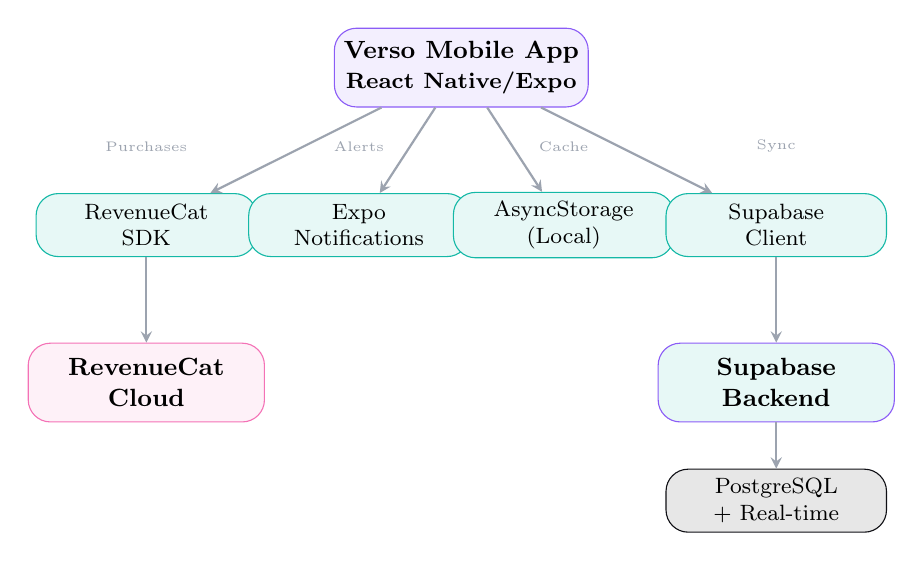
\begin{tikzpicture}[
    box/.style={rectangle, draw=versoPrimary, fill=versoPrimary!10, rounded corners=8pt, minimum width=3cm, minimum height=1cm, align=center, font=\small\bfseries},
    service/.style={rectangle, draw=versoSecondary, fill=versoSecondary!10, rounded corners=8pt, minimum width=2.8cm, minimum height=0.8cm, align=center, font=\footnotesize},
    arrow/.style={->, >=stealth, thick, color=versoMuted}
]

% Mobile App Layer
\node[box] (app) at (0,4) {Verso Mobile App\\{\footnotesize React Native/Expo}};

% Service Layer
\node[service] (rc) at (-4,2) {RevenueCat\\SDK};
\node[service] (notif) at (-1.3,2) {Expo\\Notifications};
\node[service] (storage) at (1.3,2) {AsyncStorage\\(Local)};
\node[service] (supa) at (4,2) {Supabase\\Client};

% Backend Layer
\node[box, fill=versoAccent!10, draw=versoAccent] (rcserver) at (-4,0) {RevenueCat\\Cloud};
\node[box, fill=versoSecondary!10] (supaserver) at (4,0) {Supabase\\Backend};

% Database
\node[service, fill=versoDark!10, draw=versoDark] (db) at (4,-1.5) {PostgreSQL\\+ Real-time};

% Connections
\draw[arrow] (app) -- (rc);
\draw[arrow] (app) -- (notif);
\draw[arrow] (app) -- (storage);
\draw[arrow] (app) -- (supa);
\draw[arrow] (rc) -- (rcserver);
\draw[arrow] (supa) -- (supaserver);
\draw[arrow] (supaserver) -- (db);

% Labels
\node[font=\tiny\color{versoMuted}] at (-4,3) {Purchases};
\node[font=\tiny\color{versoMuted}] at (4,3) {Sync};
\node[font=\tiny\color{versoMuted}] at (-1.3,3) {Alerts};
\node[font=\tiny\color{versoMuted}] at (1.3,3) {Cache};

\end{tikzpicture}
\end{center}

\subsection{Technology Stack}

\begin{table}[H]
\centering
\renewcommand{\arraystretch}{1.4}
\begin{tabularx}{\textwidth}{>{\bfseries}l l X}
\toprule
Layer & Technology & Purpose \\
\midrule
\multicolumn{3}{l}{\textcolor{versoPrimary}{\textbf{Frontend}}} \\
Framework & React Native 0.81 & Cross-platform mobile development \\
Meta-framework & Expo SDK 54 & Managed workflow, OTA updates, native APIs \\
Navigation & Expo Router 6 & File-based routing with deep linking \\
State & React Context & Global reminder state management \\
UI/Animations & React Native Reanimated & Fluid 60fps animations \\
\midrule
\multicolumn{3}{l}{\textcolor{versoSecondary}{\textbf{Backend Services}}} \\
Database & Supabase (PostgreSQL) & Reminders storage with RLS security \\
Real-time & Supabase Realtime & WebSocket-based live sync \\
Auth & Supabase Auth & Anonymous + email authentication \\
\midrule
\multicolumn{3}{l}{\textcolor{versoAccent}{\textbf{Monetization}}} \\
Subscriptions & RevenueCat SDK 9.7 & In-app purchases, subscription management \\
Entitlements & RevenueCat Dashboard & Pro tier feature gating \\
\midrule
\multicolumn{3}{l}{\textcolor{versoDark}{\textbf{Native Features}}} \\
Notifications & Expo Notifications & Local/push notifications with actions \\
Storage & AsyncStorage & Offline-first local persistence \\
Haptics & Expo Haptics & Tactile feedback for interactions \\
\bottomrule
\end{tabularx}
\caption{Complete Technology Stack}
\end{table}

\subsection{Directory Structure}

\begin{lstlisting}[style=typescript, title=Project Structure]
verso/
|-- app/                    # Expo Router pages
|   |-- (tabs)/            # Tab navigation screens
|   |   |-- index.tsx      # Home (Today's reminders)
|   |   |-- explore.tsx    # All reminders view
|   |-- _layout.tsx        # Root layout + providers
|   |-- modal.tsx          # New reminder modal
|   |-- edit-reminder.tsx  # Edit reminder modal
|   |-- paywall.tsx        # Subscription paywall
|   |-- settings.tsx       # User preferences
|   |-- onboarding.tsx     # First-run experience
|-- components/             # Reusable UI components
|-- context/               # React Context providers
|   |-- RemindersContext.tsx  # Global state
|-- services/              # API & SDK integrations
|   |-- revenuecat.ts     # RevenueCat integration
|   |-- supabase.ts       # Cloud sync service
|   |-- storage.ts        # Local persistence
|   |-- notifications.ts  # Push notification service
|-- types/                 # TypeScript definitions
|-- constants/             # Theme & configuration
\end{lstlisting}

% ============================================
% SECTION 3: CORE FEATURES ARCHITECTURE
% ============================================
\section{Core Features Architecture}

\subsection{Reminder Data Model}

The reminder system is built on a comprehensive data model supporting all required features:

\begin{lstlisting}[style=typescript, title=types/reminder.ts]
interface Reminder {
  id: string;                    // Local unique identifier
  syncId?: string;               // Cloud sync identifier
  title: string;                 // Reminder title
  notes?: string;                // Optional description
  datetime: string;              // ISO 8601 date string
  
  // Completion tracking
  isCompleted: boolean;
  completedAt?: string;
  
  // Recurrence configuration
  recurrence?: RecurrenceRule;
  
  // Custom snooze presets
  snoozePresets: SnoozePreset[];
  snoozedUntil?: string;
  
  // Organization
  priority: 'low' | 'medium' | 'high';
  tags?: string[];
  
  // Sync metadata
  deviceId?: string;
  createdAt: string;
  updatedAt: string;
}

type RecurrenceType = 
  | 'none' | 'hourly' | 'daily' 
  | 'weekly' | 'monthly' | 'yearly' | 'custom';

interface RecurrenceRule {
  type: RecurrenceType;
  interval: number;           // e.g., every 2 days
  daysOfWeek?: number[];      // 0-6 for weekly
  dayOfMonth?: number;        // 1-31 for monthly
  endDate?: string;
  repeatCount?: number;
}
\end{lstlisting}

\subsection{State Management Flow}

\begin{center}
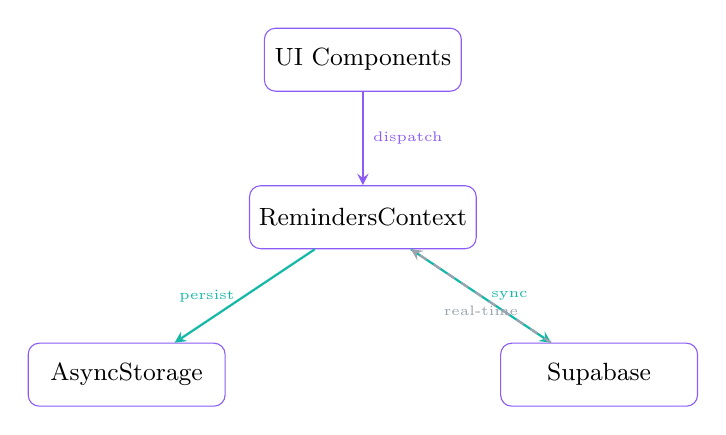
\begin{tikzpicture}[
    node distance=1.5cm,
    block/.style={rectangle, draw=versoPrimary, fill=white, rounded corners=4pt, minimum width=2.5cm, minimum height=0.8cm, font=\small},
    arrow/.style={->, >=stealth, thick}
]

\node[block] (context) at (0,0) {RemindersContext};
\node[block] (local) at (-3,-2) {AsyncStorage};
\node[block] (cloud) at (3,-2) {Supabase};
\node[block] (ui) at (0,2) {UI Components};

\draw[arrow, color=versoPrimary] (ui) -- node[right, font=\tiny] {dispatch} (context);
\draw[arrow, color=versoSecondary] (context) -- node[left, font=\tiny] {persist} (local);
\draw[arrow, color=versoSecondary] (context) -- node[right, font=\tiny] {sync} (cloud);
\draw[arrow, color=versoMuted, dashed] (cloud) -- node[below, font=\tiny] {real-time} (context);

\end{tikzpicture}
\end{center}

The \texttt{RemindersContext} acts as the single source of truth, implementing:

\begin{itemize}
    \item \textbf{Optimistic updates}: UI updates immediately while sync happens in background
    \item \textbf{Offline-first}: Changes persist locally before cloud sync
    \item \textbf{Conflict resolution}: Cloud state wins on timestamp conflicts
    \item \textbf{Real-time subscriptions}: Instant updates across devices
\end{itemize}

\subsection{Custom Snooze System}

\begin{successbox}[Key Feature: Notification Snooze]
Users can snooze reminders directly from notifications with configurable presets---a core requirement from Sam Beckman's brief.
\end{successbox}

\begin{lstlisting}[style=typescript, title=Default Snooze Presets]
const DEFAULT_SNOOZE_PRESETS: SnoozePreset[] = [
  { id: '5min',  label: '5 minutes',  minutes: 5 },
  { id: '15min', label: '15 minutes', minutes: 15 },
  { id: '30min', label: '30 minutes', minutes: 30 },
  { id: '1hr',   label: '1 hour',     minutes: 60 },
  { id: '3hr',   label: '3 hours',    minutes: 180 },
  { id: 'tomorrow', label: 'Tomorrow', minutes: 1440 },
];
\end{lstlisting}

Pro users can create custom snooze presets (e.g., ``22 minutes'') through the settings screen, fulfilling the requirement for flexible rescheduling options.

% ============================================
% SECTION 4: REVENUECAT INTEGRATION
% ============================================
\section{RevenueCat Integration \& Monetization}

\subsection{Integration Overview}

Verso uses RevenueCat SDK v9.7.5 (\texttt{react-native-purchases}) for all monetization:

\begin{table}[H]
\centering
\renewcommand{\arraystretch}{1.3}
\begin{tabularx}{\textwidth}{>{\bfseries}l X}
\toprule
Component & Details \\
\midrule
SDK Version & \texttt{react-native-purchases} ^9.7.5 \\
Platform Keys & Separate API keys for iOS and Android \\
Entitlement & ``pro'' --- unlocks all premium features \\
Offerings & Monthly, Yearly (best value), Lifetime \\
\bottomrule
\end{tabularx}
\end{table}

\subsection{SDK Initialization}

\begin{lstlisting}[style=typescript, title=services/revenuecat.ts - Initialization]
import Purchases, { LOG_LEVEL } from 'react-native-purchases';
import { Platform } from 'react-native';

const API_KEYS = {
  ios: 'appl_xxxxxxxxxxxxx',
  android: 'goog_xxxxxxxxxxxxx',
};

export async function initializeRevenueCat(): Promise<void> {
  // Skip in Expo Go (requires development build)
  if (isExpoGo()) {
    console.log('RevenueCat disabled in Expo Go');
    return;
  }

  try {
    Purchases.setLogLevel(LOG_LEVEL.DEBUG);
    const apiKey = Platform.OS === 'ios' 
      ? API_KEYS.ios 
      : API_KEYS.android;
    
    await Purchases.configure({ apiKey });
    console.log('RevenueCat initialized successfully');
  } catch (error) {
    console.error('RevenueCat init error:', error);
  }
}
\end{lstlisting}

\subsection{Subscription Status Management}

\begin{lstlisting}[style=typescript, title=Subscription Status Check]
interface SubscriptionStatus {
  isProUser: boolean;
  activeSubscription?: string;
  expirationDate?: Date;
}

export async function getSubscriptionStatus(): Promise<SubscriptionStatus> {
  const customerInfo = await Purchases.getCustomerInfo();
  
  // Check for active "pro" entitlement
  const isProUser = customerInfo
    .entitlements.active['pro'] !== undefined;
  
  if (isProUser) {
    const proEntitlement = customerInfo.entitlements.active['pro'];
    return {
      isProUser: true,
      activeSubscription: proEntitlement.productIdentifier,
      expirationDate: new Date(proEntitlement.expirationDate),
    };
  }
  
  return { isProUser: false };
}
\end{lstlisting}

\subsection{Purchase Flow Implementation}

\begin{center}
\begin{tikzpicture}[
    node distance=0.8cm and 2cm,
    block/.style={rectangle, draw=versoPrimary, fill=versoPrimary!10, rounded corners=4pt, minimum width=2.8cm, minimum height=0.7cm, font=\footnotesize, align=center},
    arrow/.style={->, >=stealth, thick, color=versoMuted}
]

\node[block] (paywall) {User opens\\Paywall};
\node[block, right=of paywall] (fetch) {Fetch\\Offerings};
\node[block, right=of fetch] (select) {Select\\Package};
\node[block, below=of select] (purchase) {Call\\purchasePackage};
\node[block, left=of purchase] (verify) {RevenueCat\\Validates};
\node[block, left=of verify] (unlock) {Unlock\\Pro Features};

\draw[arrow] (paywall) -- (fetch);
\draw[arrow] (fetch) -- (select);
\draw[arrow] (select) -- (purchase);
\draw[arrow] (purchase) -- (verify);
\draw[arrow] (verify) -- (unlock);

\end{tikzpicture}
\end{center}

\begin{lstlisting}[style=typescript, title=Purchase Package Function]
export async function purchasePackage(
  pkg: PurchasesPackage
): Promise<CustomerInfo | null> {
  try {
    const { customerInfo } = await Purchases.purchasePackage(pkg);
    return customerInfo;
  } catch (error: any) {
    if (error.userCancelled) {
      console.log('User cancelled purchase');
    } else {
      console.error('Purchase error:', error);
    }
    return null;
  }
}
\end{lstlisting}

\subsection{Subscription Tiers \& Features}

\begin{table}[H]
\centering
\renewcommand{\arraystretch}{1.4}
\begin{tabularx}{\textwidth}{l c c}
\toprule
\textbf{Feature} & \textbf{Free Tier} & \textbf{Pro Tier} \\
\midrule
Basic Reminders & \textcolor{versoSecondary}{\faIcon{check}} & \textcolor{versoSecondary}{\faIcon{check}} \\
Standard Snooze Presets & \textcolor{versoSecondary}{\faIcon{check}} & \textcolor{versoSecondary}{\faIcon{check}} \\
\midrule
Unlimited Reminders & \textcolor{versoMuted}{\faIcon{times}} & \textcolor{versoSecondary}{\faIcon{check}} \\
Cloud Sync & \textcolor{versoMuted}{\faIcon{times}} & \textcolor{versoSecondary}{\faIcon{check}} \\
Custom Snooze Presets & \textcolor{versoMuted}{\faIcon{times}} & \textcolor{versoSecondary}{\faIcon{check}} \\
Advanced Recurrence & \textcolor{versoMuted}{\faIcon{times}} & \textcolor{versoSecondary}{\faIcon{check}} \\
Theme Customization & \textcolor{versoMuted}{\faIcon{times}} & \textcolor{versoSecondary}{\faIcon{check}} \\
Home Screen Widgets & \textcolor{versoMuted}{\faIcon{times}} & \textcolor{versoSecondary}{\faIcon{check}} \\
\bottomrule
\end{tabularx}
\caption{Free vs Pro Feature Comparison}
\end{table}

\subsection{Restore Purchases}

\begin{lstlisting}[style=typescript, title=Restore Purchases Implementation]
export async function restorePurchases(): Promise<CustomerInfo | null> {
  try {
    const customerInfo = await Purchases.restorePurchases();
    return customerInfo;
  } catch (error) {
    console.error('Restore error:', error);
    return null;
  }
}

// Usage in Paywall
const handleRestore = async () => {
  const customerInfo = await restorePurchases();
  if (customerInfo) {
    const status = await getSubscriptionStatus();
    if (status.isProUser) {
      Alert.alert('Restored!', 'Your purchase has been restored.');
    }
  }
};
\end{lstlisting}

% ============================================
% SECTION 5: CLOUD SYNC ARCHITECTURE
% ============================================
\section{Cloud Sync Architecture}

\subsection{Supabase Integration}

\begin{infobox}[True Cross-Device Sync]
Verso implements real-time sync via Supabase, ensuring that ``dismissing once clears everywhere''---a key requirement from the brief.
\end{infobox}

\subsubsection{Database Schema}

\begin{lstlisting}[style=typescript, title=PostgreSQL Schema (supabase-schema.sql)]
CREATE TABLE reminders (
    id UUID PRIMARY KEY DEFAULT uuid_generate_v4(),
    user_id UUID REFERENCES auth.users(id) ON DELETE CASCADE,
    title TEXT NOT NULL,
    notes TEXT,
    datetime TEXT NOT NULL,
    is_completed BOOLEAN DEFAULT FALSE,
    completed_at TEXT,
    priority TEXT DEFAULT 'medium',
    recurrence JSONB,
    snooze_presets JSONB DEFAULT '[]'::JSONB,
    snoozed_until TEXT,
    device_id TEXT,
    created_at TEXT DEFAULT NOW()::TEXT,
    updated_at TEXT DEFAULT NOW()::TEXT
);

-- Row Level Security (RLS)
ALTER TABLE reminders ENABLE ROW LEVEL SECURITY;

CREATE POLICY "Users can view own reminders"
    ON reminders FOR SELECT
    USING (auth.uid() = user_id);

-- Enable real-time subscriptions
ALTER PUBLICATION supabase_realtime ADD TABLE reminders;
\end{lstlisting}

\subsection{Real-Time Sync Flow}

\begin{center}
\begin{tikzpicture}[
    device/.style={rectangle, draw=versoPrimary, fill=versoPrimary!10, rounded corners=8pt, minimum width=2cm, minimum height=1.5cm, align=center},
    cloud/.style={ellipse, draw=versoSecondary, fill=versoSecondary!10, minimum width=3cm, minimum height=1.5cm, align=center},
    arrow/.style={<->, >=stealth, thick, color=versoMuted}
]

\node[device] (iphone) at (-3,0) {\faIcon{apple}\\iPhone};
\node[device] (android) at (3,0) {\faIcon{android}\\Android};
\node[cloud] (supa) at (0,0) {Supabase\\Real-time};

\draw[arrow] (iphone) -- (supa);
\draw[arrow] (android) -- (supa);

\node[font=\tiny\color{versoMuted}] at (-1.5,0.8) {WebSocket};
\node[font=\tiny\color{versoMuted}] at (1.5,0.8) {WebSocket};

\end{tikzpicture}
\end{center}

\begin{lstlisting}[style=typescript, title=Real-Time Subscription Handler]
// Subscribe to real-time changes
Supabase.subscribeToReminders(
  // Handle remote inserts
  (reminder: Reminder) => {
    if (!reminders.some(r => r.syncId === reminder.syncId)) {
      setReminders(prev => [...prev, reminder]);
    }
  },
  // Handle remote updates
  (reminder: Reminder) => {
    setReminders(prev => prev.map(r => 
      r.syncId === reminder.syncId ? reminder : r
    ));
  },
  // Handle remote deletes
  (syncId: string) => {
    setReminders(prev => 
      prev.filter(r => r.syncId !== syncId)
    );
  }
);
\end{lstlisting}

\subsection{Conflict Resolution Strategy}

\begin{table}[H]
\centering
\renewcommand{\arraystretch}{1.3}
\begin{tabularx}{\textwidth}{>{\bfseries}l X}
\toprule
Scenario & Resolution \\
\midrule
Simultaneous edits & Latest \texttt{updatedAt} timestamp wins \\
Offline changes & Queued locally, synced on reconnection \\
New device & Full merge with existing cloud data \\
Delete conflicts & Delete propagates if newer than last update \\
\bottomrule
\end{tabularx}
\end{table}

% ============================================
% SECTION 6: SECURITY
% ============================================
\section{Security Architecture}

\subsection{Authentication Flow}

\begin{enumerate}
    \item \textbf{Anonymous Auth}: Users start with anonymous Supabase auth (no friction)
    \item \textbf{Email Upgrade}: Optional email/password for account recovery
    \item \textbf{Session Persistence}: Tokens stored securely via AsyncStorage adapter
\end{enumerate}

\subsection{Row Level Security (RLS)}

All database operations are protected by PostgreSQL RLS policies:

\begin{lstlisting}[style=typescript, title=RLS Policies]
-- Users can only access their own data
CREATE POLICY "Users can view own reminders"
    ON reminders FOR SELECT
    USING (auth.uid() = user_id);

CREATE POLICY "Users can insert own reminders"
    ON reminders FOR INSERT
    WITH CHECK (auth.uid() = user_id);

CREATE POLICY "Users can update own reminders"
    ON reminders FOR UPDATE
    USING (auth.uid() = user_id);

CREATE POLICY "Users can delete own reminders"
    ON reminders FOR DELETE
    USING (auth.uid() = user_id);
\end{lstlisting}

% ============================================
% SECTION 7: PERFORMANCE
% ============================================
\section{Performance Optimizations}

\begin{itemize}[leftmargin=*]
    \item[\faIcon{bolt}] \textbf{Optimistic UI Updates}: Instant feedback before network confirmation
    \item[\faIcon{database}] \textbf{Local-First Architecture}: App works fully offline
    \item[\faIcon{sync}] \textbf{Incremental Sync}: Only changed records are transferred
    \item[\faIcon{memory}] \textbf{Memoized Computations}: Filtered lists computed with \texttt{useMemo}
    \item[\faIcon{film}] \textbf{60fps Animations}: React Native Reanimated for smooth transitions
\end{itemize}

% ============================================
% SECTION 8: BUILD & DEPLOYMENT
% ============================================
\section{Build \& Deployment}

\subsection{Development Builds}

\begin{lstlisting}[style=typescript, title=Build Commands]
# Development build for iOS
npx expo run:ios

# Development build for Android  
npx expo run:android

# EAS Build for TestFlight/Play Store
eas build --platform ios --profile production
eas build --platform android --profile production
\end{lstlisting}

\subsection{Environment Configuration}

\begin{table}[H]
\centering
\begin{tabularx}{\textwidth}{l X}
\toprule
\textbf{File} & \textbf{Purpose} \\
\midrule
\texttt{app.json} & Expo configuration, app identifiers, splash screens \\
\texttt{eas.json} & EAS Build profiles (development, preview, production) \\
\texttt{tsconfig.json} & TypeScript compiler configuration \\
\bottomrule
\end{tabularx}
\end{table}

% ============================================
% SECTION 9: ROADMAP
% ============================================
\section{Future Roadmap}

\begin{featurebox}
\textbf{Post-Hackathon Development Priorities}

\begin{enumerate}
    \item \textbf{iOS Widgets}: Home screen widgets for quick reminder access
    \item \textbf{Apple Watch App}: Glanceable reminders on wrist
    \item \textbf{Location-Based Triggers}: ``Remind me when I arrive at...''
    \item \textbf{Siri/Google Assistant}: Voice-activated reminder creation
    \item \textbf{Shared Lists}: Collaborative reminders for families/teams
    \item \textbf{Web Dashboard}: Browser access for power users
\end{enumerate}
\end{featurebox}

% ============================================
% APPENDIX
% ============================================
\appendix
\section{API Reference}

\subsection{RevenueCat Service Functions}

\begin{table}[H]
\centering
\renewcommand{\arraystretch}{1.3}
\begin{tabularx}{\textwidth}{>{\ttfamily}l X}
\toprule
\textnormal{\textbf{Function}} & \textbf{Description} \\
\midrule
initializeRevenueCat() & Configure SDK with platform-specific API key \\
getOfferings() & Fetch available subscription packages \\
purchasePackage(pkg) & Initiate purchase flow for selected package \\
restorePurchases() & Restore previous purchases on new device \\
getSubscriptionStatus() & Check current entitlement status \\
setUserId(id) & Associate user ID for cross-platform sync \\
\bottomrule
\end{tabularx}
\end{table}

\subsection{Dependencies}

\begin{table}[H]
\centering
\footnotesize
\renewcommand{\arraystretch}{1.2}
\begin{tabularx}{\textwidth}{l l X}
\toprule
\textbf{Package} & \textbf{Version} & \textbf{Purpose} \\
\midrule
react-native-purchases & ^9.7.5 & RevenueCat SDK \\
@supabase/supabase-js & ^2.93.3 & Supabase client \\
expo-notifications & ~0.32.16 & Push notifications \\
expo-router & ~6.0.21 & File-based navigation \\
react-native-reanimated & ~4.1.1 & Animations \\
date-fns & ^4.1.0 & Date manipulation \\
\bottomrule
\end{tabularx}
\end{table}

% ============================================
% FOOTER
% ============================================
\vfill
\begin{center}
\textcolor{versoMuted}{\rule{0.5\textwidth}{0.5pt}}

\vspace{0.5cm}

{\Large\textcolor{versoPrimary}{\faIcon{bell}} \textbf{Verso}}

\textcolor{versoMuted}{Cross-Platform Power Reminders}

\vspace{0.3cm}

\textcolor{versoMuted}{\small Built for RevenueCat Shipyard: Creator Contest 2026}

\textcolor{versoMuted}{\small Sam Beckman Brief}
\end{center}

\end{document}
